
% IEEES 2020 conference format checklist:
% - to check!
% FORMAT: 
%            - roman numbers for sections, how do I change it?
%            - fix references parenthesis style (see notes in reference section)



%Fonts are typically available only in certain sizes/increments. As an example, the basic article document class loads only the following sizes (from size10.clo):

 %   \tiny @ 5pt;
 %   \scriptsize @ 7pt;
 %   \footnotesize @ 8pt;
 %   \small @ 9pt;
 %   \normalsize @ 10pt;
 %  \large @ 12pt;
 %   \Large @ 14.4pt;
 %   \LARGE @ 17.28pt;
 %   \huge @ 20.74pt; and
 %   \Huge @ 24.88pt


%%%%%%%%%%%%%%%%%%%%%%%%%%%%%%%%%%%%%%%%%%

\documentclass[10pt]{extarticle} %extendend font dimensions
\usepackage[margin=2cm,top=1cm,bottom=2cm]{geometry}
%\usepackage{helvet}
%\renewcommand{\familydefault}{\sfdefault}

%\usepackage[pass,showframe]{geometry}
\usepackage{amsmath}
\usepackage[english]{babel}
% author year bibliography  
\usepackage{natbib}

% Use of [T1]{fontenc}
% If you don't use \usepackage[T1]{fontenc}:
% - Words containing accented characters cannot be automatically hyphenated,
% - You cannot properly copy-and-paste such words from the output (DVI/PS/PDF),
% - Characters like the pipe sign, less than and greater sign give unexpected results.
\usepackage[T1]{fontenc}

\usepackage{newtxtext,newtxmath}

%%%%%%%%%% image packages:

\usepackage{graphicx}

\usepackage[export]{adjustbox}

\usepackage{subcaption}


%%%%%%%%%%%%%%%%%%%%%%%%%%

\renewcommand{\sfdefault}{phv} %makes arial the default font for sff

\newcommand{\bigsize}{\fontsize{12pt}{16pt}\selectfont} %12pt dim/ 16pt spacing

\newcommand{\subsecsize}{\fontsize{10pt}{10pt}\selectfont} %14pt dim 

\newcommand{\namesize}{\fontsize{10pt}{10pt}\selectfont} %13pt dim 

\usepackage[sf,pagestyles]{titlesec} % make section headings \sffamily

% headings formats:

\titleformat{\section}[block]
            {\sffamily\normalsize\bfseries}
            {\thesection.}{6pt}{\filright}
            
\titleformat{\subsection}[block]
            {\sffamily\subsecsize\bfseries}
            {\thesubsection.}{6pt}{\filright}

\titleformat{\subsubsection}[block]
            {\sffamily\subsubsecsize\bfseries}
            {\thesubsubsection.}{6pt}{\filright}

%% https://tex.stackexchange.com/questions/326331/titleformat-problem


%title format:-----------------------
\usepackage{titling} % make titling elements \sffamily
\pretitle{\begin{center}\sffamily\bigsize\textbf}
\preauthor{\begin{center}
            \small\sffamily\ \lineskip 0.5em%
            \begin{tabular}[t]{c}}
%------------------------------------

% abstract format:-------------------
\usepackage{abstract}
% make abstract title \sffamily

\renewcommand\abstractnamefont{\sffamily\normalsize\bfseries}
\renewcommand{\abstracttextfont}{\sffamily\normalsize}
\renewcommand{\absnamepos}{raggedleft}
\setlength{\absleftindent}{0cm}
\setlength{\absrightindent}{0cm}

% ------------------------------------

%\bibliographystyle{vancouver}
\bibliographystyle{plainnat}

\title{The dead state of buildings}
\author{Valentina Bonetti\\ University of Strathclyde, Department of Mechanical and Aerospace Engineering, 75 Montrose St, Glasgow, G1 1XJ,  UK\\ \\ E-mail: valentina.bonetti@strath.ac.uk}

\date{}

% NOTES ABOUT ARTICLE CONTENT:

% - REFER	 to SalaLizarraga2020 chapter of book for summary of meaning and ref environment requirement (part of the problem or background)

% keep reading WEPFER GAGGIOLI 1979-80 "Reference datums for available energy"


\begin{document}
\renewcommand{\abstractname}{Abstract:}



\begin{figure}[!h]
\centering

\includegraphics[width=6.8in, center]{images/articleHeading1.png}
\end{figure}

%\maketitle
\let\newpage\relax
\vspace*{-2cm}
\maketitle
\vspace*{-1cm}


\begin{abstract}

\noindent Exergy is typically defined as the maximum work that can be extracted from a system when reaching equilibrium with its ``reference environment'' - a large region unaffected by the interactions - and derives from Gibbs' original concept of ``available energy of a body and medium''. The reference environment definition  plays a key role in exergy analysis but is still controversial, especially in the case of buildings; the most popular choice is the local outdoor air, because readily available and largely unaffected by the presence of the building, but its fluctuating conditions pose various challenges. The controversy around the reference environment arguably remains one of the main blockers in the practical application of building exergy methods.
However, going back to the origins, Gibbs defined available energy not only for a ``body and medium'', but also for the case of a ``body alone'', a system formed by subsystems in non-equilibrium conditions. Later, exergy too was defined for this second case, as the subsystem contribution to the body available energy. In the case of the ``body alone'', the reference is the ``dead state'' (the thermostatic condition of the body), in place of the reference environment. 
The main idea of this article is that building exergy analysis can be based not only, as currently, on the exergy definion originated by Gibbs' case of the ``body and medium'', but alternatively on the exergy definition originated by the case of the  ``body alone'', for which a large environment is not needed.  The outdoor reference environment can thus be substituted by an indoor ``dead state''. 
The study discusses possible system boundaries and ways of defining the building dead state based on indoor conditions, and the potential impact on building exergy analysis. The dynamic exergy modelling of a few cases is presented to visualise the numerical implications.

\end{abstract}

\noindent {\sffamily\normalsize\bfseries Keywords:}
{\sffamily\normalsize Exergy, reference environment, dynamic analysis.}


\section{Introduction} 

\sffamily\normalsize

% SUGGESTIONS:
%Help the reader understand why your research is important and what it is contributing to the field:
%Start by giving the reader a brief overview of the current state of research in your subject area.
%Progress to more detailed information on the specific topic of your research.
%End with a description of the exact question or hypothesis that your paper will address.
%Also state your motivation for doing your research and what it will contribute to the field.

% Preamble (horrible, write it better)
Debating the reference of exergy analysis requires going back to the beginning, and investigating where its requirements originated. 
% Gibbs
\cite{Gibbs1873} was the first to combine the first and second law of thermodynamics in one equation \citep{Klein1990}, in his first paper "Graphical methods in the Thermodynamics of Fluids".  The combination of the first and second law of thermodynamics led Gibbs to introduce the concept of ``available energy"; he distinguished two cases: a "body alone", in internal non-equilibrium conditions, and a "body and medium", in non-equilibrium conditions with each other. 

In the case of the ``body alone", the available energy of the body is the greatest amount of mechanical work that ideally can be obtained by taking the body, without any net contributions of energy from external objects, from its initial non-equilibrium condition to the point of stable or neutral equilibrium (on the ``surface of dissipated energy") that has the same entropy and volume of the initial state. The internal non-equilibrium state of the body can assume various forms, like a difference in the pressure of some of its part, or a gradient in temperature, or even different chemical compositions. It is important to observe that the term ``body" refers not necessarily to a single entity but to a system potentially including several subsystems and processes \citep{Gaggioli2012}.
 
In the case of the ``body and medium", the medium is supposed to be at constant pressure and constant temperature. The medium is also called ``reference environment", a large subsystem that is not affected by the interactions with the other components of the overall system, and it is represented by a plane in Gibbs' graphical representation of the energy-entropy-volume space. The available energy in this case is the distance (on the energy axis) from the point corresponding to the initial conditions of the body to the point on the medium plane with the same entropy and volume. Even if the body is in internal equilibrium, the combination between body and medium can still have available energy, unless they are in the same conditions. 


%Present some of fundamental Gaggioli equations for exergy.
\cite{Gaggioli2012} provided a definition of the ``dead state" based on Gibbs' ``available energy of a body" (the first case mentioned above)  that does not require a reference environment. 

\vfill \break

\section{The dead state of a very simple building} \label{subsec:simple}

Discuss an insulated cave with no air exchanges and negligible internal gains. Simulate it on the side and present image.


 
\begin{figure}[h]
 
\begin{subfigure}{0.35\textwidth}
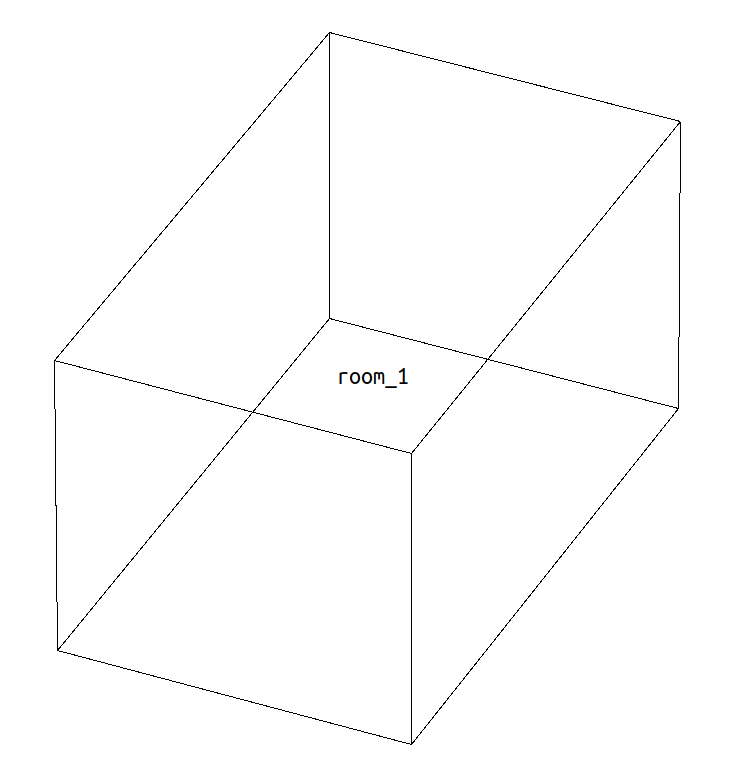
\includegraphics[width=0.95\linewidth, height=6cm]{images/Dead02_boxModel.png} 
\caption{ESP-r box model.}
\label{fig:esprmodel}
\end{subfigure}
\begin{subfigure}{0.65\textwidth}
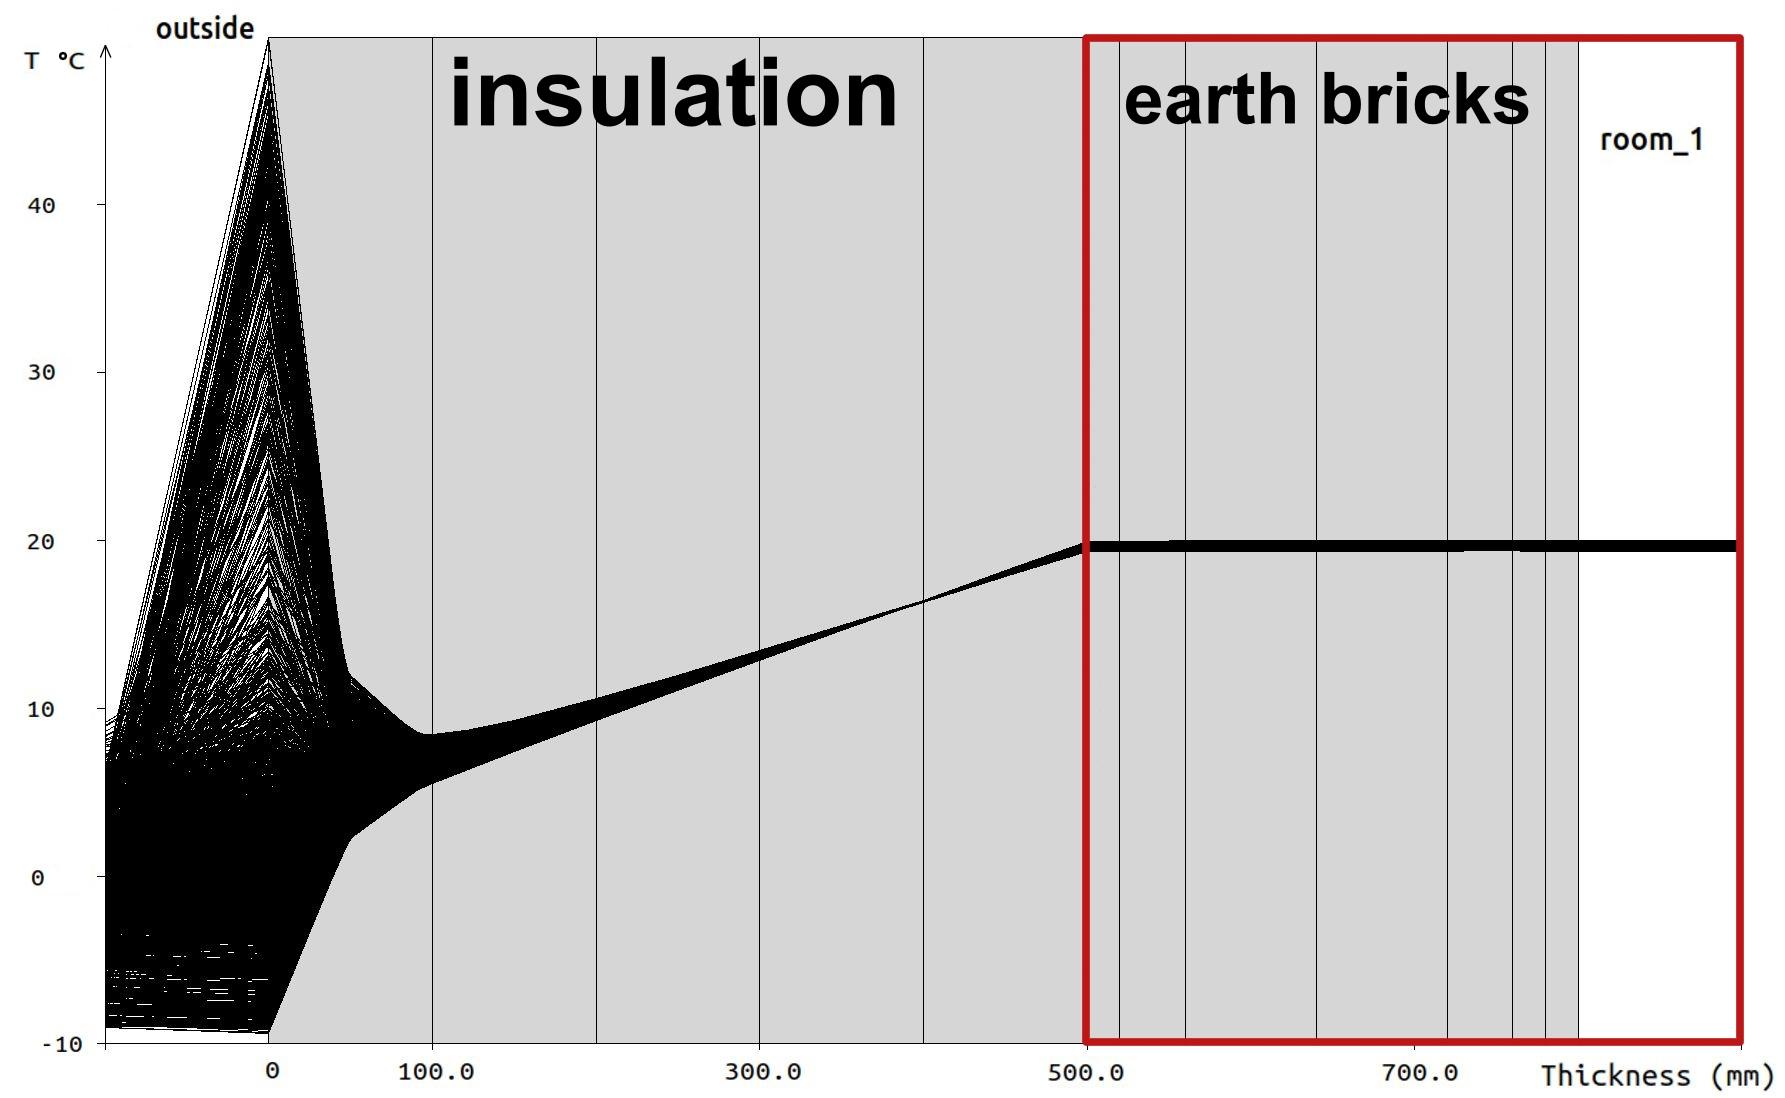
\includegraphics[width=0.95\linewidth, height=6cm]{images/01Feb_28Feb_Wall1_dead02_krita.jpg}
\caption{Cumulative values of intra-construction temperatures in a wall of the box model.}
\label{fig:constructionelements}
\end{subfigure}
 
\caption{The first case study: a box model with 500 mm of exterior  insulation and 300 mm of earth on the internal layers.}
\label{fig:casestudy}
\end{figure}




\vskip3cm


\vfill \break


\section{A more realistic case} \label{subsec:moreComplex}

Statement about the importance of internal loads, not only for summer but also on heating strategies. 
Include window and internal gains. Simulate on the side and present image. Still very good insulation.
Also present increasingly complex cases, with air exchanges and lower insulation, mainly visually.
Define the "core" of the envelope (periodic penetration depth) and specify that it is a first attempt definition.

{\bf Calculate instantaneous dead state and compare with target dead state. Do a sensitivity analysis of typical quantities involved.}

\vskip3cm


\section{Dead state and design goals}

In most cases the core of the building envelope is far from an isolated system, but the indoor environment has a comfort target nevertheless. When the HVAC system is switched off, we expect the indoor conditions to remain comfortable for as long as possible, and as soon as they fall out of an acceptable range the heating or cooling system intervenes again to bring temperature and sometimes also relative humidity back to the required values. In other words, it is like if the composition of the overall system changed dynamically to include subsystems capable of re-establishing the desired dead state. Sometimes the external environment has the exergy that the building needs to maintain its conditions, for instance cooler air could be let in to readdress internal gains, or solar radiation could enter from fenestration to compensate transmission losses. When the balance cannot be maintained by passive design strategies, an exergy input from renewable or non-renewable sources is required. In any case, the final destination is an indoor environment very close to, or going towards, comfort conditions, with a multitude of exergy fluxes and storages being orchestrated to balance each other with the goal of a comfortable dead state.

The core of the building, including the internal part of the envelope and the indoor environment, might have both warm and cool exergy storages, which both contribute to the overall exergy, in this case also "available energy". A greater available energy is an expression of disequilibrium, and potentially of a greater effort needed to maintain comfort conditions. Zero available energy indicates that the system is in uniform comfort conditions, because all the exergy contributions are positive.




\vfill \break

\section{Conclusions and future work}
Wall insulation is relatively easy - main challenges today are indoor comfort and thermal storage / decoupling energy demand and offer (just my opinion though, look for references). Indoor dead state shifts the focus on the indoor environment.

\section*{Acknowledgments}

The author thanks the Engineering and Physical Sciences Research Council U.K. (EPSRC, Grant No.1586601) and the Building Research Establishment (BRE) for the financial support.

{\small %font size 9
 \bibliography{ValeIEEES2020}
}
%% Max 10-15 refs
% NOTES FOR BIBLIOGRAPHY
% References“Arial, 10 points, bold”
% “Arial, 9 points, alphabetic order of names (first author), max 10-15 important references.”
% “If Mendeley is used, you can select Journal of Cleaner Production or similar referencing styles”

\vfill \break

%
%\subsection{Exergy storage} \label{subsubsec:basicEq_exergystorage}
%
%The exergy stored in a portion of matter of uniform properties is expressed per unit volume by the following equation, in which the subscript n indicates a generic node:
%
%\begin{equation}
%\label{exergystoragenode}
%ex_n = c_n \rho_n \left[ \left( T_n - T_0 \right) - T_0 \ln {T_n\over T_0} \right]
%\approx {{c_n\rho_n \left(T_n-T_0 \right)^2 \over 2 T_0}}
%\end{equation}
%
%\noindent with $c_n$ specific heat, $\rho_n$ density and $T_n$ temperature of matter, and $T_0$ reference temperature. Equation \ref{exergystoragenode} is clearly positive for any value of node and reference temperatures, since any state different from the reference can theoretically produce work, but the stored exergy assumes different meanings \cite{Shukuya2013} depending on their relationship:
%
%\begin{itemize}
%\item if $T_n > T_0$ it is called "warm exergy";
%\item if $T_n < T_0$ it is called "cool exergy";
%\item if $T_n = T_0$ the exergy stored is null and the node is at the reference state.
%\end{itemize}
%
%\noindent To make the distinction between cool and warm exergy, the sign function sgn is used to equation \ref{exergystoragenode}, which becomes:
%\begin{equation}
%\label{exergystoragenodewithsign}
%ex_n \approx sgn(T_n-T_0)\cdot {{c_n\rho_n \left(T_n-T_0 \right)^2 \over 2 T_0}}
%\end{equation}
%This is why in the graphs of \ref{subsec:casestudy} a cool exergy will be shown as negative (in blue) and a warm exergy storage will appear as positive (red). The value of $ex_n$ is then multiply by the volume of each layer to obtain the actual storage.
%
%\subsection{Exergy of air flow} \label{subsubsec:basicEq_exergyAirFlow}
%
%The exergy carried by air at a volume flow rate of $\dot{V}$ and temperature $T_{air}$, with specific heat at constant pressure $c_{p,air}$ and density $\rho_{air}$, is calculated in a similar way:
%\begin{equation}
%\label{exergyflowair}
%\dot{Ex}_{air} = c_{p,air} \rho_{air} \dot{V} \left[ \left( T_{air} - T_0 \right) - T_0 \ln {T_{air}\over T_0} \right]
%\end{equation}
%
%\noindent The total exergy transported in a period $[t_1,t_2]$ is simply obtained through the integral:
%
%\begin{equation}
%\label{totalexergyflowair}
%Ex_{air} = \int_{t_1}^{t_2} c_{p,air} \rho_{air} \dot{V} \left[ \left( T_{air} - T_0 \right) - T_0 \ln {T_{air}\over T_0} \right] dt
%\end{equation}
%
%
%
%\section{Case study} \label{subsec:casestudy}
%
%A simple three-zone building is considered as a case study, and only one zone (the office in Fig.\ref{fig:casestudy}) is analised. The weather file is the "default UK Climate" of the dynamic software ESP-r, and a few typical winter days are considered (6th to 8th of February). ESP-r uses a finite-volume approach, which makes it possible to calculate the temperature values of nodes within constructions for each timestep. The construction elements surrounding the office zone are subdivided in a different number of layers (from 1 of the internal door to 8 of the floor), and each layer is composed of three nodes. The heating loads are covered by an ideal Constant Air Volume (CAV) system activated from 7am to 6pm, with two possible settings described in section \ref{exergyOfHeating}, and the building is left in a free-floating mode outside of this range.
% 
%\begin{figure}[h]
% 
%\begin{subfigure}{0.4\textwidth}
%\includegraphics[width=0.95\linewidth, height=6cm]{images/ESPrBasicModel.png} 
%\caption{ESP-r model and office zone.}
%\label{fig:esprmodel}
%\end{subfigure}
%\begin{subfigure}{0.6\textwidth}
%\includegraphics[width=0.9\linewidth, height=6cm]{images/00_ESPrOfficeSurfacesListTrimmed.png}
%\caption{Construction elements defining office zone.}
%\label{fig:constructionelements}
%\end{subfigure}
% 
%\caption{The case study: office zone of a simple building with an average-performing envelope.}
%\label{fig:casestudy}
%\end{figure}
%
%An example snapshot of the temperature of each node within the construction elements is reported in Fig.\ref{fig:nodetemperatures} for the first timestep of the simulation. The number of nodes vary from 3 (single-layer door) to 17 of the floor.  The performance of the case-study construction is relatively poor, but the particular values are not relevant for the purposes of the present research. 
%The temperature of the first node of each construction element is the temperature of the inner surfaces surrounding the zone, and thus have a direct impact on the occupant comfort, depending also on the area of the surfaces, their view factors and optical properties. %does the view factor already include the area? don't think so, but check!
%
%\begin{figure}[!h]
%\centering
%\includegraphics[width=4in]{images/01_tempCon02_time_000.png}
%\caption{Temperature ($^\circ$C) for each node of the 8 envelope elements of the office zone (timestep 0).}
%\label{fig:nodetemperatures}
%\end{figure}
%\vskip0.6cm
%
%
%\subsection{Exergy stored in construction layers}
%
%The exergy stored in each layer of the envelope elements surrounding the office zone is calculated for each timestep, according to equation \ref{exergystoragenode}. For the sake of simplicity, the central temperature of each layer is used in the equation as the temperature of the entire layer. A better approximation would be considering a linear trend for the temperature inside the half of each layer, interpolating the node temperatures, but for the aims of this study such accuracy is not necessary\footnote{It is also easily possible to increment the number of layers of the ESP-r model, if a better calculation of the exergy storage is needed.}.
%
%The values of exergy are highly affected by the choice of the reference state, as discussed in section \ref{subsec:basicExergyEq}. Figure \ref{fig:exsto_000} shows the difference for a snapshot taken at timestep 0; the exergy storage based on a fixed reference state $T_0=T_{0,fixed}=20^\circ$C is "cool exergy" for every node of the zone construction elements (in blue in Fig. \ref{fig:exstofixed_000}), whilst the opposite holds true for the exergy storage calculated with the variable reference, $T_0=T_{0,variable}[0]=2.2^\circ$C at the first timestep (red "warm exergy" in Fig. \ref{fig:exstovariable_000}). 
%
%\begin{figure}[h]
% 
%\begin{subfigure}{0.5\textwidth}
%\includegraphics[width=0.95\linewidth, height=6cm]{images/01_ExergyConStorage_Fixed_time_000_edges.png} 
%\caption{Fixed reference state, timestep 0.}
%\label{fig:exstofixed_000}
%\end{subfigure}
%\begin{subfigure}{0.5\textwidth}
%\includegraphics[width=0.95\linewidth, height=6cm]{images/01_ExergyConStorage_Variable_time_000_edges.png}
%\caption{Variable reference state, timestep 0.}
%\label{fig:exstovariable_000}
%\end{subfigure}
% 
%\caption{Exergy stored in construction layers (Wh), office zone.}
%\label{fig:exsto_000}
%\end{figure}
%
%
%The inner layers of the envelope (numbers 1 on the bottom of the graphs in Figs. \ref{fig:exstofixed_000} and \ref{fig:exstovariable_000}) interact with the indoor environment directly, and thus the exergy stored within these elements provides an idea of their dynamic behaviour and impact on indoor comfort. If, for example, "cool exergy" is stored in the inner layer of a wall at the timestep $t$, the layer will provide a "cooling effect" on the indoor environment, which duration in time depends on the entity of the storage and speed of response on the exergy quality factor. The other layers of the envelope are obviously still important, as they determine the conditions of the inner layers and a relevant amount of their exergy will be transmitted to the indoor space on the longer term. It is worth observing that the definition of "inner layer" is rather vague in this study because it just derives, for the sake of simplicity, from the energy model subdivision of the envelope elements, which does not contemplate any exergy considerations in its design. A deeper effort on the definition of a more meaningful inner layer size should be included in further investigations. 
%
%A qualitative idea of the trends of inner-layer exergy storage for the entire duration of the case-study simulation is provided in Fig.\ref{fig:exstoindoornodes_alltimes}. Figure \ref{fig:exstofixed_indoornodes_alltimes} on the left shows the exergy storage based on a fixed reference state: the partition walls have a negligible impact in terms of storage (because their temperature is very near to the reference but also because of their lightweight construction), the rest of the layers have a moderate cooling effect. The exergy storage based on the variable reference, shown in Fig.\ref{fig:exstovariable_indoornodes_alltimes}, tells a different story; the partition walls still have an almost null impact (mainly due to their low mass) but the other envelope elements provide a "warm storage" at any timestep, with a higher variablility (the peak value, in absolute terms, is approximately six times bigger than the peak predicted by the fixed reference).
%
%\begin{figure}[h]
% 
%\begin{subfigure}{0.5\textwidth}
%\includegraphics[width=0.99\linewidth, height=7cm]{images/02_exStoIndoorConNodes_Fixed_alltimes.png} 
%\caption{Fixed reference}
%\label{fig:exstofixed_indoornodes_alltimes}
%\end{subfigure}
%\begin{subfigure}{0.5\textwidth}
%\includegraphics[width=0.99\linewidth, height=7cm]{images/02_exStoIndoorConNodes_Variable_alltimes.png}
%\caption{Variable reference}
%\label{fig:exstovariable_indoornodes_alltimes}
%\end{subfigure}
% 
%\caption{Exergy stored in construction indoor layers (Wh), office zone.}
%\label{fig:exstoindoornodes_alltimes}
%\end{figure}
%
%
%A more quantitative visualisation of the inner-envelope exergy storage is provided by the graph of the sum of the exergy stored in all the inner layers for each timestep. 
%Figure \ref{fig:exstofixed__indoorsum_day3} reports the values based on a fixed reference state for day 3 of the simulation, and shows how the cool exergy stored in the envelope diminishes during the periods of active heating and internal gains (hours 55 to 66, corresponding to 7am to 6pm) and is moderately influenced by the outdoor climate (slow cool exergy increase during the periods 00am to 7am -52h to 55h- and after 6pm, caused by the heat transfer on the outer side of the layer). The values calculated with a variable reference state, reported in Fig.\ref{fig:exstovariable_indoorsum_day3}, are remarkably more affected by the outdoor temperature: the warm exergy increases during a period when the inner layers become colder, because the outdoor temperature is decreasing at a faster rate, and the entire trend shadows the outdoor temperature variations (observable in Fig.\ref{fig:exergyofair} of section \ref{subsec:ventilationair}).
%
%
%\begin{figure}[h]
% 
%\begin{subfigure}{0.5\textwidth}
%\includegraphics[width=0.95\linewidth, height=5.5cm, center]{images/05_TotInsideExStoConLayer_Fixed_day3.png} 
%\caption{Fixed reference}
%\label{fig:exstofixed__indoorsum_day3}
%\end{subfigure}
%\begin{subfigure}{0.5\textwidth}
%\includegraphics[width=0.95\linewidth, height=5.5cm, center]{images/05_TotInsideExStoConLayer_Variable_day3.png}
%\caption{Variable reference}
%\label{fig:exstovariable_indoorsum_day3}
%\end{subfigure}
% 
%\caption{Exergy stored in all construction indoor layers (Wh), 8th of February (day 3), office zone.}
%\label{fig:exsto_indoorsum_day3}
%\end{figure}
%
%\subsection{Exergy of fresh air intake} \label{subsec:ventilationair}
%
%Different terminology is used to indicate the outdoor air entering the zone. ESP-r defines "infiltration" air the sum of all naturally-induced air flows and mechanical ventilation coming from outside the building, and "ventilation" the air movement between different thermal zones; various other source use the term "ventilation" to indicate intentional intake of outdoor air and "infiltration" for unintentional fluxes of the same air. In this study, the second terminology is used because clearer to a wider audience, and thus "ventilation and infiltration" indicates the sum of all fresh air intake from the outdoor environment, and the movement between zones is simply called "air from other zone".
%
%In the case-study model, the rate of fresh air intake of the office zone ($V_{zone}=48m^3$) is fixed at 0.3 air changes per hour (ACH), which means a volumetric flow rate of $\dot{V} = ACH \cdot V_{zone} / 3600\ s = 0.3\cdot 1/h\cdot 48m^3\cdot (1/3600)s/h=0.004 {m^3/s}$. The properties of air are considered constant at $c_{p,air}=1006\ J/(kg K)$ and $\rho_{air}=1.2\ kg/m^3$. These values are substituded in equation \ref{exergyflowair} to obtain the graph in Fig.\ref{fig:exergyofair}.
%
%
%\begin{figure}[!h]
%\centering
%\includegraphics[width=4in]{images/06_InfiltrationExergyRatePlusT_8Feb.png}
%\caption{Exergy of the fresh air intake, fixed and variable reference; indoor and outdoor T (office, day 3).}
%\label{fig:exergyofair}
%\end{figure}
%\vskip0.6cm
%
%The outdoor air temperature is below the indoor temperature (and the heating setpoint at 20$^\circ$C) for the entire period, and thus the fresh air intake represents a heating load. The exergy calculation based on a fixed reference classifies the air flow as a "cool" exergy contribution to the zone, whilst from the point of view of the variable reference the flow appears as neutral (zero exergy). 
%
%\subsection{Exergy of the heating system} \label{exergyOfHeating}
%
%The heating loads of the case study are covered by an ideal Constant Air Volume (CAV) system, and two possible settings are explored:
%
%\begin{itemize}
%\item maximum air temperature $T_{CAV,max} = 30^\circ$C and constant air rate $\dot{V}_{CAV} = 0.04\ m^3/s$
%\item maximum air temperature $T_{CAV,max} = 50^\circ$C and constant air rate $\dot{V}_{CAV} = 0.02\ m^3/s$
%\end{itemize}
%
%\noindent The exergy rate of the CAV flow is calculated with the same Eq.\ref{exergyflowair} of the fresh air flow. The variable temperature of the heating system CAV T is provided by the ESP-r software and is reported in Fig. \ref{fig:CAV} for both settings. The second option, illustrated in Fig.\ref{fig:CAV_50_002}, has a higher exergy factor but a lower air flow rate than the first option of Fig.\ref{fig:CAV_30_004}.
%
%Since the CAV air temperature is higher than both the comfort and outdoor temperature, all the calculated exergy flows are positive, representing a warm exergy contribution to the zone for both the fixed and variable reference state.  When the maximum temperature is lowered to $30^\circ$C, the system is slower in reaching a comfortable indoor temperature even with a doubled air flow rate. If a variable reference state is adopted, low-exergy systems values are particularly affected by the variation of the outdoor temperature. The variable-reference exergy line of the graph in Fig.\ref{fig:CAV_30_004} clearly mirrors the outdoor temperature, and a lighter mirroring effect is visible in the case of variable-reference curve of the higher-exergy system in Fig.\ref{fig:CAV_50_002}. These effects are not observable in the fixed-reference curves, which clearly reflect only the CAV temperature trends.
%
%
%\begin{figure}[h]
% 
%\begin{subfigure}{0.5\textwidth}
%\includegraphics[width=0.95\linewidth, height=6cm, center]{images/04_CAV_30_004_ExergyRatePlusT_day3.png} 
%\caption{CAV T max $30^\circ$C, Constant flow rate $0.04\ m^3/s$}
%\label{fig:CAV_30_004}
%\end{subfigure}
%\begin{subfigure}{0.5\textwidth}
%\includegraphics[width=0.95\linewidth, height=6cm, center]{images/04_CAV_50_002_ExergyRatePlusT_day3.png}
%\caption{CAV T max $50^\circ$C, Constant flow rate $0.02\ m^3/s$}
%\label{fig:CAV_50_002}
%\end{subfigure}
% 
%\caption{Exergy flow of Constant Air Volume (CAV) system, 8th of February (day 3), office zone.}
%\label{fig:CAV}
%\end{figure}
%
%
%
%% Report integral (total exergy) values in the two CAV cases.
%The total exergy contribution over a defined period is calculated with Eq.\ref{totalexergyflowair}, which represents the area below the exergy rate function. The values obtained for the two CAV options are:
%
%\begin{itemize}
%\item for CAV $30^\circ$C, $0.04\ m^3/s$: \\ $Ex_{CAV,fixed}[52h,68h] = 46.47\ Wh$, \quad $Ex_{CAV,variable}[52h,68h] = 481.1\ Wh$
%\item for CAV $50^\circ$C, $0.02\ m^3/s$: \\ $Ex_{CAV,fixed}[52h,68h] = 133.4\ Wh$, \quad $Ex_{CAV,variable}[52h,68h] = 478.3\ Wh$
%\end{itemize}
%
%
%The exergy analysis performed with a fixed reference shows a significative difference between the two options: the low-temperature case demands a lower exergy, in terms of peak value but also of total Wh, and therefore the low-exergy system appears slower but able to mantain a comfortable indoor environment with a much lower exergy consumption (approximately one third). On the other hand, the analysis based on a variable reference does not provide a clear distinction, because although the  $50^\circ$C CAV exergy rate peak is around 30\% higher than the  $30^\circ$C maximum exergy rate, the total exergy carried over the sample day is approximately the same.
%
%
%
%
%
%\subsection{Energy and exergy demand} \label{sub:EnergyExergyDemand}
%
%The most influential terms of the daily energy balance (related to day 3 of the case-study simulation) are presented in Fig.\ref{fig:EnergyCausalBreakdown}. The total heating loads and the sum of ventilation and infiltration are also shown as instantaneous values in Fig.\ref{fig:TotHeatInfLosses}, because needed for the calculation of the "detailed exergy demand" based on the variable reference state, as defined in the following section \ref{detailedHeatExDemand}. The simplified calculation of the exergy demand proposed by the present study, presented in section \ref{subsub:fixedExergyDemand}, does not require the instantaneous breakdown of thermal loads explicitly. 
%
%
%\begin{figure}[h]
% 
%\begin{subfigure}{0.5\textwidth}
%\includegraphics[width=0.95\linewidth, height=6.3cm, center]{images/ZoneEnergyBalance2_Merged_Office_8Feb.png} 
%\caption{Causal breakdown of energy balance (kWh)}
%\label{fig:EnergyCausalBreakdown}
%\end{subfigure}
%\begin{subfigure}{0.5\textwidth}
%\includegraphics[width=0.95\linewidth, height=6.3cm, center]{images/07_HeatingAndVentilationLoads.png}
%\caption{Total heating and ventilation+infiltration loads (W)}
%\label{fig:TotHeatInfLosses}
%\end{subfigure}
% 
%\caption{Energy overall balance and detailed heating and ventilation plus infiltration loads (day 3, office).}
%\label{fig:EnergyBalance}
%\end{figure}
%
%\subsubsection{Detailed exergy demand} \label{subsub:detailedExDemand}
%
%The "detailed" exergy demand defined by the IEA Annex 49 \cite{Schmidt2011} is divided in two components: $Ex_{dem,vent}$ is the part attributed to an ideal pre-heating of the ventilation air and the remaining part $Ex_{dem,heat}$ is the exergy of the total loads minus the part that is preheated through the ventilation ($Q_{dem,heat}=Q_{dem,total}-Q_{dem,vent}$)\footnote{If the ventilation plus infiltration loads are greater than the overall loads, than a pre-heating temperature lower than the heating setpoint needs to be calculated; in the present case study the total heating loads are greater than the ventilation loads at any timestep, and therefore the pre-heating temperature calculation is not needed. See \cite{Schmidt2011} for further details.}. Each component is calculated according to:
%
%\begin{equation}
%\label{detailedVentExDemand}
%Ex_{dem,vent}=Q_{dem,vent}\cdot \left( 1 - {T_0\over T_{preheat}-T_0} \ln {T_{preheat}\over T_0} \right)
%\end{equation}
%
%\begin{equation}
%\label{detailedHeatExDemand}
%Ex_{dem,heat}=Q_{dem,heat}\cdot \left( 1 - {T_0\over T_{room}} \right) 
%\end{equation}
%
%\noindent where the reference temperature $T_0$ is the variable outdoor air temperature, $Q_{dem,total}$ and $Q_{dem,vent}$ are the instantaneous loads illustrated in Fig.\ref{fig:TotHeatInfLosses} and $Q_{dem,heat}$ their difference, and $T_{preheat}$ coincides in this case with the office air temperature $T_{room}$. The total detailed exergy demand for the day 3 under analysis (8th of February), obtained by integration of the instantaneous values, is:
%
%\begin{itemize}
%\item Exergy demand to heat ventilation air up to the zone temperature: $Ex_{dem,vent} = 21.6\ Wh$
%\item Exergy demand to supply heat as heat at zone temperature: $Ex_{dem,heat}= 166\ Wh$
%\end{itemize}
%
%If based on the fixed reference state $T_{0,fixed}$ as defined in this study, both components of this detailed exergy demand result null.
%
%\subsubsection{Exergy demand based on comfort as the fixed reference} \label{subsub:fixedExergyDemand}
%
%The exergy demand calculated with the fixed reference state based on comfort is null at comfort temperature by definition. This means that the ideal minimum exergy demand of any building is zero and is constituted by a very large amount (theoretically infinite, if the comfort state was exactly defined) of energy at the comfort state.
%
%The definition of a heating or cooling system, although still ideal, is needed in order to calculate a more pragmatic exergy demand: without an active system, the building is not actually  "capable of asking" for exergy. The smallest exergy demand based on the fixed reference is therefore linked to following step of the building chain: the emission system. 
%
%In the particular case study presented here, the emission-system exergy demand on day 3 of the simulation coincides with the quantities calculated in section \ref{exergyOfHeating} with the fixed reference:
%
%\begin{itemize}
%\item $Ex_{dem,emission}(CAV 30^\circ C, 0.04\ m^3s^{-1}) = 46.47\ Wh$
%\item $Ex_{dem,emission}(CAV 50^\circ C, 0.02\ m^3s^{-1}) =  133.4\ Wh$
%\end{itemize}
%
%It is not surprising that there are different values of exergy demand depending on the emission system. An ideal system demanding less exergy can always be found, since the minimum demand is null, but this is not necessarily the design target.
%
%
%
%
%\section{Conclusions and future work} % 0.5 pages --------
%
%
%In pragmatic terms, if "warm" exergy is simply what is above the middle line of an indoor comfort range and "cool" exergy what is below, understanding exergy becomes remarkably simpler.
%More complex fixed reference states could be certainly be thought of, maybe based on an ideal comfortable building (contemplating a range of temperatures for the zone air, a range for the interior surfaces, a range of humidity and other human comfort parameters, and probably a significant average of these ranges) but the impact on the comparison between the fixed and the variable reference state frameworks would me marginal. A first "good-enough" and robust approach could recognise exergy analysis as probably best fitted for building design and policies (and not for metering), without requiring a very high accuracy in order to provide useful information but simple enough to be widely adopted. 
% 
%The usefulness of exergy lies in the fact that every source becomes directly comparable, and it is possible to make informed decisions about interesting issues, such as strategies for renewable energy intergration or electrification of heat. For example, the exergy factors within comfort levels indicate "very low-exergy" energies that are able to "mantain" the state within the range, making it possible to use the indoor environment as a source and sink of internal energy interactions (which are not infinite). These "slow" energies could even be directly controlled by energy providers, since the time of their release is not critical (the user just need to define the desired comfort range). Thermal exergies well outside the comfort range are instead used for faster heating and cooling interventions. High-exergy fluxes like electricity are more flexible because their release time can be modified, making them fast or slow sources. 
%
%
%
%
%%In particular, we will be able to quantify the real waste, which needs to be compatible with the actual budget, not only in economical but also in environmental terms.
%
%
%
%
%% Keep the following section-titles unchanged to comply with ECOS conference format!
%
%
%
%
%
%
%
%
%



\end{document}




% LaTeX references:

% Use of package [T1]{fontenc}: 
% https://tex.stackexchange.com/questions/664/why-should-i-use-usepackaget1fontenc

% https://tex.stackexchange.com/questions/25249/how-do-i-use-a-particular-font-for-a-small-section-of-text-in-my-document

% abstract package documentation:
% http://citeseerx.ist.psu.edu/viewdoc/download?doi=10.1.1.169.8953&rep=rep1&type=pdf

% title formats using titlesec:
% http://mirror.ox.ac.uk/sites/ctan.org/macros/latex/contrib/titlesec/titlesec.pdf
% https://tex.stackexchange.com/questions/326331/titleformat-problem

